\documentclass{report} \usepackage[T1]{fontenc} \usepackage[italian]{babel}
\usepackage{color}
\usepackage[type={CC},modifier={by-sa},version={4.0},]{doclicense}
\usepackage{cite}

\usepackage{graphicx}
\graphicspath{ {./media/images/} }
\usepackage{float}
\usepackage{subcaption}

\usepackage{hyperref}

\addto\captionsitalian{\renewcommand{\bibname}{Riferimenti}}

\title{Title} \author{Daniele Melocchi\\Agnese Montanaro\\Matteo
Savatteri}

\begin{document}
\maketitle
\setcounter{page}{2}

Copyright Daniele Melocchi, Agnese Montanaro, Matteo Savatteri -
\the\year \doclicenseThis \thispagestyle{empty}

\tableofcontents

\chapter{Introduzione}
Questo documento presenta un ciclo di lezioni svolte in modalità
di didattica a distanza (\emph{DAD}) e
indirizzate ad una classe 1\textsuperscript{a} Liceo Scientifico,
riguardanti le basi della cinematica, il moto rettilineo uniforme
e uniformemente accelerato.

Il percorso didattico è suddiviso in tre moduli, all'interno dei quali
sono affrontati i seguenti argomenti, ordinati secondo un criterio
di complessità crescente, partendo da un approccio completamente
qualitativo, per passare ad uno via via più quantitativo:
\begin{enumerate}
\item Posizioni, istanti, distanze e intervalli temporali, leggi orarie.
\item Velocità media, velocità istantanea, moto rettilineo uniforme.
\item Accelerazione media, accelerazione istantanea, moto uniformemente
      accelerato.
\end{enumerate}

Il percorso si fonda sul \emph{modello didattico delle 5E}\cite{bybee2006bscs}.
Ogni modulo si suddivide dunque in cinque fasi, nelle quali sono presentate
attività, riflessioni, suggerimenti e problematiche affrontate, per ciascuna
di queste: \emph{engage}, \emph{explore}, \emph{explain}, \emph{extend},
\emph{evaluate}.

\section{Propedeuticità}
Al fine della buona riuscita di questo percorso, è necessario che gli
studenti coinvolti abbiano affrontato e consolidato la comprensione
dei seguenti argomenti:
\begin{itemize}
\item Operazioni algebriche elementari (es. frazioni e potenze).
\item Polinomi.
\item Equazioni di primo grado.
\item Rappresentazioni di numeri su un asse ordinato.
\item Rappresentazione di coppie di numeri (punti) su un diagramma
      cartesiano.
\item Conoscenza di grandezze fondamentali.
      (es. lunghezza, tempo)
\item Conoscenza di unità di misura di grandezze fondamentali.
      (es. metro, secondo)
\end{itemize}

\chapter{Posizioni, Istanti, Distanze, Intervalli Temporali} \label{posizioni_istanti}
Nel presente modulo lo studente familiarizza con i concetti
di posizione, distanza, istante (inteso come
\emph{lettura di orologio}) e intervallo di tempo.
Succesivamente, guidato dal docente, esplora le relazioni
che intercorrono tra queste nozioni nel contesto del moto di
un corpo, giungendo ad una comprensione qualitativa dei
concetti di \emph{evento} e \emph{legge oraria}.

\section{Engage}
\begin{itemize}
\item \textbf{Tempo richiesto in aula:} 15\textsuperscript{$\prime$}
\item \textbf{Materiale:} Computer
\end{itemize}

Il docente mostra agli studenti
\footnote{
Nel contesto della DAD, il docente può utilizzare
una piattaforma web di videotelefonia, che supporti la condivisione
di file multimediali. Jitsi Meet\textsuperscript{\textregistered},
Zoom\textsuperscript{\textregistered},
Google Meet\textsuperscript{\textregistered} e
Microsoft Teams\textsuperscript{\textregistered}
sono solo alcuni esempi.
}
il video di un fenomeno fisico riprodotto \emph{in reverse} (ovvero ribaltando
l'asse temporale). Il fenomeno fisico rappresentato dovrebbe essere scelto
in modo che sia difficile (o impossibile) distinguere se il video viene
riprodotto in reverse oppure no. Il moto di un pendolo semplice,
di un \emph{pendulum wave} o di altri moti periodici costituiscono buoni
esempi.

Nel contesto di questo progetto si è scelto il video in \emph{slow motion}
di un colibrì in volo, che si nutre da un tubicino (Figura \ref{fig:hummingbird})
\footnote{
\`E possibile scaricare il video presso
\href{https://github.com/savaroskij/PED1/blob/master/progetto_finale/media/video/Hummingbird.mp4?raw=true}{questa pagina web}
. L'indirizzo del video originale si trova nei riferimenti\cite{hbird}.
}.
Solamente la componente video, e non quella audio, è stata invertita per
aumentare l'effetto di inganno.

\begin{figure}
\centering
  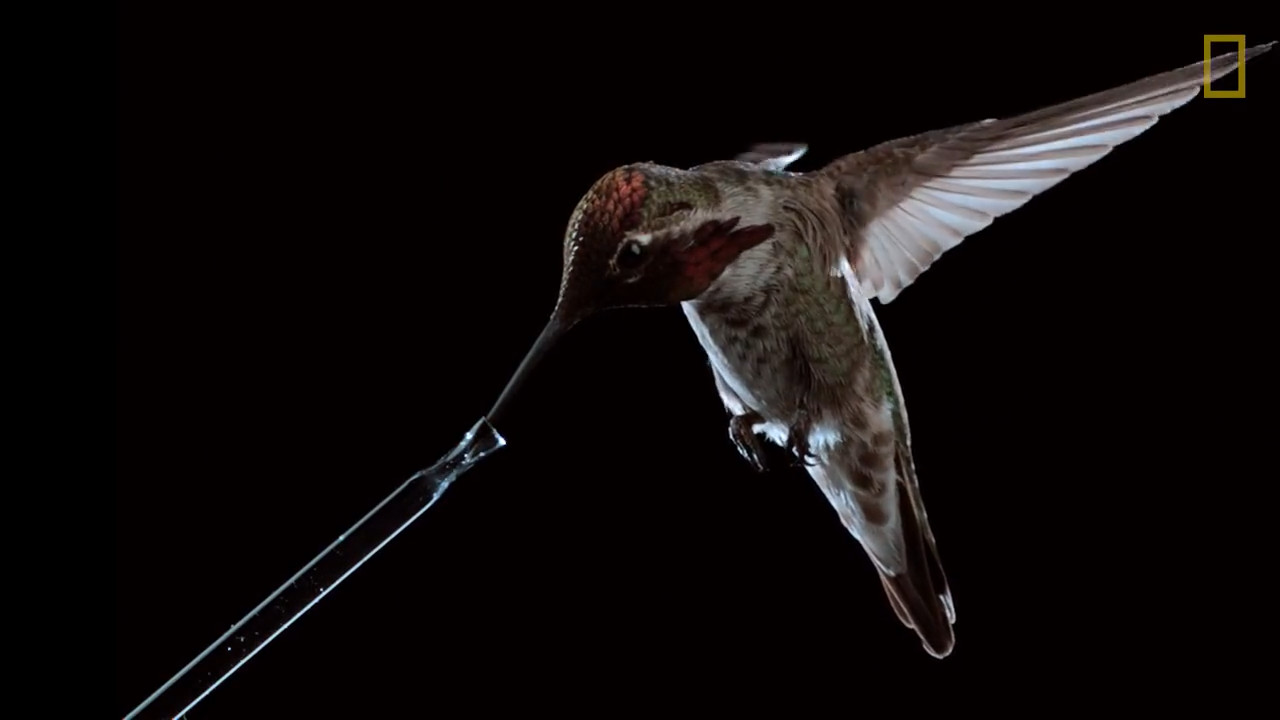
\includegraphics[width=\textwidth]{Hummingbird}
  \caption{Un frame del video di un colibrì in volo che si nutre da un tubicino.}
  \label{fig:hummingbird}
\end{figure}

Il docente in seguito chiede agli studenti di descrivere quanto viene
visualizzato, e solamente infine svela che il video è riprodotto in
reverse. In questo modo l'insegnante ha l'occasione di far notare
allo studente, e lo esplicita, che per studiare qualsiasi fenomeno fisico
occorrono chiari riferimenti spaziali e temporali.

\section{Explore}
Questa fase viene svolta da ciascun studente a casa. Il professore propone agli
alunni tre attività distinte, attraverso le quali possano arrivare a
comprendere i concetti citati precedentemente (Inizio Capitolo \ref{posizioni_istanti}).

In primo luogo gli
studenti dovrebbero cogliere il significato di istante di tempo, o meglio
\emph{lettura di orologio}\cite{arons1997teaching}
\footnote{
           Il linguaggio utilizzato dal docente deve essere il più chiaro possibile, in modo
           che lo studente possa non fraintendere i concetti. Per esempio utilizzare il
           termine momenti, invece che letture di orologio, rimanda lo studente ad un
           concetto di tempo prolungato, non di istante.
         }
, e la differenza con intervallo
di tempo e in secondo luogo il significato di posizione e la differenza con distanza.
Tutte e tre le attività si basano sull’utilizzo della fotografia
\footnote{
          \`E opportuno che il tempo di esposizione per un singolo scatto sia ridotto, al
            fine di cogliere il concetto di istante temporale.
         }
e di grafici.

Emerge dalla letteratura, infatti, che l’utilizzo di grafici risulta essere un
ottimo strumento per la comprensione di concetti di base della cinematica
\cite{beichner1994testing}. I grafici possono essere
utili sia per descrivere il moto di un corpo osservato sia per prevedere il tipo
di moto a partire dal grafico stesso.

\subsection{Fotografare nel Tempo}

\begin{itemize}
\item \textbf{Materiale richiesto:} Smartphone, Fogli di Carta
\item \textbf{Tempo richiesto in aula:} 10\textsuperscript{$\prime$}
\end{itemize}

La prima attività proposta consiste nel fotografare diversi moti o situazioni
(minimo 3) scelti dallo studente in vari momenti (possono essere scattate sia
nella stessa giornata che in giorni differenti), quindi disegnare una linea del
tempo su un foglio e posizionare le foto scattate secondo i momenti scelti. Non
occorre scegliere una scala per la linea del tempo, perché interessa che lo
studente si accorga solo qualitativamente del fatto che possano passare periodi
di tempo di diversa durata tra eventi diversi. Inoltre in questa attività si
dovrebbe cogliere che il tempo ha una propria sequenzialità e che ciascuna
fotografia è un evento che accade in un istante determinato di tempo.

\`E opportuno che il docente guidi gli studenti mostrando loro un paio di esempi
di quanto richiesto, come una sequenza di foto di una pentola piena d’acqua
posta sul fuoco o episodi di vita quotidiana (Figura \ref{fig:asse_t_pentola}).

\begin{figure}[H]
\centering
  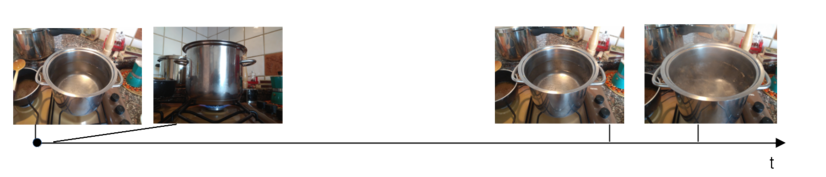
\includegraphics[width=\textwidth]{asse_t_pentola}
  \caption{Istanti del fenomeno di una pentola piena d'acqua posta sul fuoco,
           collocati sulla linea del tempo.}
  \label{fig:asse_t_pentola}
\end{figure}

\subsection{Fotografare nello Spazio}

\begin{itemize}
\item \textbf{Materiale richiesto:} Smartphone, Foglio di Carta
\item \textbf{Tempo richiesto in aula:} 10\textsuperscript{$\prime$}
\end{itemize}

Come seconda attività viene chiesto di scegliere un punto di partenza su un
corso o una via ed esplorarla camminando, fotografando palazzi o altri oggetti
incontrati (almeno 3 oggetti distinti). In seguito si disegni una linea su un
foglio e si incollino le diverse fotografie in base alla disposizione dei
soggetti immortalati lungo la via. Anche in questo caso non occorre che la
linea presenti una scala, in quanto l’obiettivo del lavoro è comprendere il
concetto di posizione di un corpo nello spazio e, in modo qualitativo, della
posizione relativa rispetto ad altri oggetti.

Anche in questo caso occorre che il professore mostri almeno uno più esempi
(Si veda la Figura \ref{fig:asse_s}).

\begin{figure}[H]
\centering
  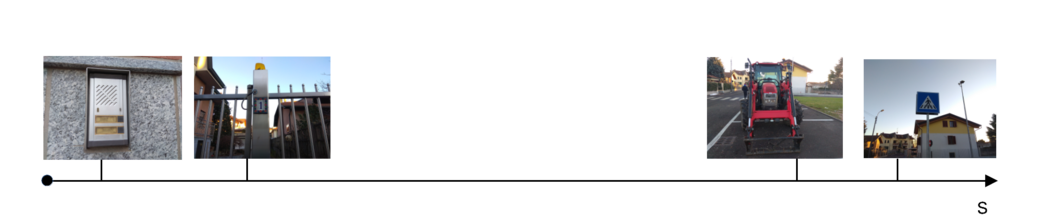
\includegraphics[width=\textwidth]{asse_s}
  \caption{Vari oggetti immortalati lungo una via e rappresentati
           sulla linea della posizione.}
  \label{fig:asse_s}
\end{figure}

\subsection{Fotografarsi nel Tempo e nello Spazio}

\begin{itemize}
\item \textbf{Materiale richiesto:} Smartphone, Foglio di Carta
\item \textbf{Tempo richiesto in aula:} 10\textsuperscript{$\prime$}
\end{itemize}

Infine, la terza attività consiste nel ripercorrere (dall'inizio alla fine
senza mai tornare idietro) la medesima via della
seconda esperienza, scattando dei \emph{selfie} e appuntandosi la lettura di orologio
corrispondente a ciascuna foto. Viene richiesta una elaborazione grafica in
analogia a quanto fatto nelle precedenti, senza che l’insegnante ne specifichi
la struttura finale.

Il professore per questa terza attività mostrerà solamente le fotografie
scattate, senza mostrare agli studenti il grafico ottenuto, in modo che gli
studenti possano ragionare su questo caso più complicato.
Gli studenti dovrebbero essere in grado di capire che per rappresentare
un corpo (loro stessi) che si muove nello spazio è necesserio utilizzare
due assi distinti, ovvero un diagramma cartesiano bidimensionale.
La Figura \ref{fig:piano_s_t} mostra un esempio del risultato atteso.

Tutte e tre le attività sono pensate per essere svolte incollando le fotografie
su un foglio, perché si ritiene che attraverso questa modalità operativa lo
studente  possa avere occasione di riflettere e giudicare i risultati ottenuti.

\begin{figure}[ht]
\centering
  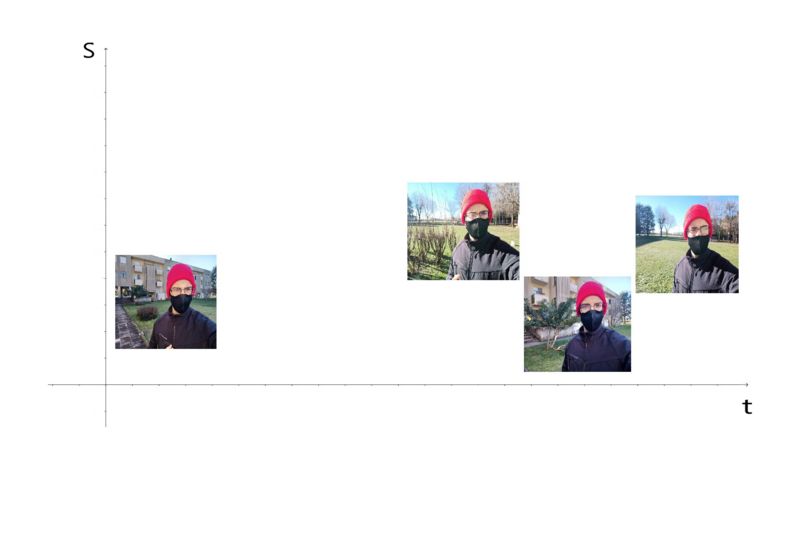
\includegraphics[width=\textwidth]{piano_s_t}
  \caption{I \emph{selfie} della terza attività, rappresentati
           su un piano cartesiano.}
  \label{fig:piano_s_t}
\end{figure}

\section{Explain}\label{posizioni_istanti_explain}
\begin{itemize}
\item \textbf{Tempo richiesto:} 20\textsuperscript{$\prime$} di discussione tra
studenti + 30\textsuperscript{$\prime$} di dialogo con il docente
\end{itemize}

In questa fase viene permesso agli alunni di confrontarsi ed interpretare
quanto svolto nella fase precedente; il professore può intervenire per spiegare
o formalizzare alcuni concetti emersi.
L’insegnante \emph{in primis} suddivide la classe in gruppi di cinque studenti
\footnote{
          Per  esperienza degli autori, un numero esiguo o eccessivo di membri
          di un gruppo di lavoro rende difficile il coinvolgimento di tutti i
          partecipanti.
         }
e assegna
ciascun gruppo ad un’aula virtuale differente. La piattaforma utilizzata sarà a
discrezione della scuola
\footnote{
          Una possibilità è la piattaforma Zoom\textsuperscript{\textregistered},
          che  permette facilmente di creare aule virtuali di lavoro.
         }.
L’insegnante chiede di
discutere i grafici ottenuti nelle attività precedenti, confrontandoli, e
visita le aule virtuali per monitorare il lavoro ed eventualmente indirizzare
lo sguardo degli alunni con alcune domande. Per esempio: ``Che cosa potreste
dire della disposizione delle fotografie? Che significato potrebbe avere?''.
Ogni gruppo inizia quindi un \emph{brainstorming} e sceglie un portavoce,
il quale ha il  compito di esporre quanto emerso di fronte alla classe riunita
in un’unica aula virtuale con il professore.

Ciascuno studente nello svolgere la prima attività dovrebbe osservare che
alcune foto potrebbero essere più ravvicinate tra loro di altre
\ref{fig:asse_t_pentola}. Si ritiene che la maggioranza
interpreti la disomogeneità della disposizione delle
immagini come corrispondente a periodi di tempo di diversa durata tra i diversi
scatti. Il professore può formalizzare questo concetto utilizzando il termine
\emph{intervallo di tempo}, lasciando che gli studenti ne diano la definizione.
Sì osserverà, l’intervallo di tempo sarà dato dalla differenza tra le
letture di orologio delle due fotografie. Il docente a questo punto può
domandare se un singolo scatto occupi un intervallo di tempo. Si ritiene che la
maggior parte degli alunni abbia chiaro che la risposta sia no. La letteratura
fa intendere che un focus importante è assicurarsi che lo studente comprenda
che un istante di tempo equivale a \emph{zero} secondi\cite{arons1997teaching}
\footnote{
          Qualche alunno potrebbe argomentare il contrario, sostenendo che un singolo scatto
          occupi un intervallo di tempo molto breve. Questa ipotesi è corretta. Tuttavia,
          il tempo di un singolo scatto risulta essere su una scala di ordini di
          grandezza inferiore rispetto a quella utilizzata per l’attività. Per questo
          motivo si assume ad istante il tempo di una fotografia.
         }.
Ciascuna fotografia corrisponde ad un istante di tempo differente.

Dopo aver discusso i risultati della prima attività, risulta più immediato il
ragionamento sulla seconda. Un maggior numero di studenti è in grado di dire
che ciascuno oggetto fotografato è in un luogo preciso, cioè occupa una
posizione definita nello spazio. Alcuni possono costruire un’analogia tra
l’intervallo di tempo tra uno scatto e l’altro della prima attività e lo spazio
tra un oggetto e l’altro in questa esperienza. Si ipotizza che qualcuno in
classe riuscirà a far corrispondere l’aver camminato tra un oggetto incontrato
e l’altro con il concetto di \emph{distanza}.

Per quanto riguarda la terza esperienza è possibile che molti studenti si siano
trovati in difficoltà nella parte di rappresentazione grafica, in quanto meno
guidata delle precedenti. Tuttavia, è plausibile che in qualche gruppo di
lavoro sia emersa almeno l’impossibilità di utilizzare un’unica linea.
L’attività, infatti, comprendeva due grandezze differenti: tempo e spazio.
Nel caso nessun componente della classe sia arrivato ad ipotizzare un grafico
con due assi, che indicano rispettivamente spazio e tempo, allora il professore
è legittimato a guidarli in questa scoperta. Egli può far notare loro la
presenza di due informazioni distinte per ciascuna foto e invitarli ad un
paragone con i risultati delle prime due attività.
Inoltre in questa attività vi è un altro aspetto che si ritiene possa emergere
dalla discussione: il soggetto fotografato. Infatti, gli studenti potrebbero
osservare che, a differenza delle prime due attività, qui il soggetto è sempre
lo stesso in ogni scatto, cambiano solo i luoghi in cui si trova e le letture
di orologio. Dunque, il grafico caratterizzato dai due assi posizione-tempo
mostra dove si trova il soggetto fissato un istante di tempo, ovvero rappresenta
il moto di questo corpo. Il professore sottolinea nuovamente l’esistenza di
due informazioni, la posizione e il tempo, e che esse siano in relazione tra
loro. Egli in particolare spiega che esse sono legate dal concetto
di \emph{legge oraria}:  una relazione che determina la posizione occupata da un
corpo  in moto (sempre il medesimo; in questa attività, sè stessi) ad un istante
fissato.

\section{Extend}
\begin{itemize}
\item \textbf{Tempo richiesto in aula:} 30\textsuperscript{$\prime$}
\item \textbf{Materiale:} Computer, Oggetti domestici
\end{itemize}

In questa fase si proprone un attività mirata ad estendere la consapevolezza
degli studente riguardo ad alcuni concetti presentati precedentemente.
In particolare si desidera estendere l'idea di posizione, che lo studente ha maturato,
allo spazio tridimensiosale.

L'insegnante chiede a ciascuno studente di scegliere un oggetto nella stanza e di
spiegare alla classe, con le proprie parole, dove questo eggetto si trovi.
Lo studente potrebbe utilizzare altri oggetti nella stanza come riferimenti spaziali,
dicendo ad esempio ``L'oggetto si trova accanto alla finestra'', oppure
``L'oggetto si trova sopra il tavolo''; o forse potrebbe utilizzare se stesso come
riferimento affermando ``L'oggetto si trova alla mia destra, in alto''.
A questo punto il docente chiede di scegliere altri due o tre oggetti,
e fa la stessa richiesta di localizzazione. Lo studente si renderà
conto dell'impossibilità di creare nella propria mente un'idea della stanza
degli altri compagni e della posizione di tutti gli oggetti, senza che
costoro esplicitino un riferimento spaziale univoco, e per ogni oggetto indichino tre distanze
misurate o stimate dal riferimento scelto.
L'insegnante dovrebbe guidare gli studenti in questo processo ponendo domande e fornendo suggerimenti
come: ``Dove si trova l'oggetto A rispetto all'oggetto B? E rispetto all'oggetto C?'',
oppure ``Dire che l'oggetto A si trova un metro sopra l'oggetto B è sufficiente
a far comprendere al tuo compagno la posizione dell'oggetto B all'interno della stanza?''
e ancora ``Forse potremmo dire che l'ogetto B si trova sopra l'oggetto A, ma anche alla sua destra
e qualche metro più avanti''.
Al termine di questo processo, il docente ufficializza la conoscenza acquisita disegnando
\footnote{
Il professore può disegnare su una lavagna e filmarsi durante l'operazione, oppure
utilizzare una tavoletta grafica o una lavagna virtuale (presente in software
come Zoom\textsuperscript{\textregistered}, ad esempio).
}
un diagramma cartesiano tridimensionale, collocando alcuni oggetti al suo interno
e osservando che la posizione dell'oggetto preso come riferimento per tutti gli altri
si chiama \emph{origine} e le tre distanze sono rappresentate da tre numeri lungo
gli assi, chiamati \emph{coordinate cartesiane} tridimensionali.

\section{Evaluate}
Per la valutazione di questo primo modulo del percorso il docente tiene conto della
partecipazione degli studenti alle varie attività proposte, del lavoro svolto sui
grafici richiesti e del loro coinvolgimento attivo all’interno dei gruppi di discussione.

\chapter{Velocità, Moto Rettilineo Uniforme}
In questa fase lo studente verrà guidato alla comprensione del concetto di
velocità media e istantanea, e di legge oraria di un moto rettilineo
uniforme attraverso alcune attività. Occorre che il percorso sia guidato, perché
gli studenti di prima liceo affrontano per la prima volta questi argomenti e
il \emph{modus operandi} della fisica.

\section{Engage}

\begin{itemize}
\item \textbf{Tempo richiesto in aula:} 15\textsuperscript{$\prime$}
\item \textbf{Materiale:} Liquidi di Differente Viscosità, Contenitori Trasparenti Identici, Biglie
\end{itemize}

L’insegnante mostra agli studenti la caduta di una biglia in diversi liquidi. \`E
possibile eseguire questo esperimento sia in DAD, mostrando in telecamera i
contenitori con i liquidi, sia in classe portando tutto il materiale
occorrente. La scelta delle sostanze utilizzate è libera. L’unico criterio importante è
che i liquidi abbiano viscosità sensibilmente diverse, poiché in questo modo la velocità
della biglia all'interno del contenitore sarà visibilmete differente nei vari casi.

In questo progetto sono state scelte le seguenti sostanze: detersivo per i piatti,
acqua e olio di semi; posti in tre contenitori di pari altezza, trasparenti e di forma
il più possibile cilindrica (così da non avere effetti ottici di deformazione della
biglia che cade) (Figura \ref{fig:liquids}).
Le biglie utilizzate devono essere tutte uguali tra loro per massa e dimensione.

\begin{figure}[H]
\centering
  \begin{subfigure}[b]{0.5\textwidth}
  
\includegraphics[width=\textwidth]{cat_caviar}
  \end{subfigure}
  \begin{subfigure}[b]{0.5\textwidth}
  
\includegraphics[width=\textwidth]{cat_caviar}
  \end{subfigure}
  \begin{subfigure}[b]{0.5\textwidth}
  
\includegraphics[width=\textwidth]{cat_caviar}
  \end{subfigure}
  \caption{
           I tre contenitori riempiti con i liquidi
           scelti per l'attività di engage sulla
           velocità: detersivo, acqua, olio di semi.
          }
  \label{fig:liquids}
\end{figure}

Prima di iniziare la fase operativa, il professore propone un gioco
agli studenti, chiedendo loro di indovinare in quale liquido la biglia
si muoverà più velocemente. \`E importante che in questa fase e per
tutto il resto del percorso didattico, il docente non utilizzi termini
che si riferiscono a concetti che gli studenti non hanno mai
affrontato prima. \`E necessario infatti che lo studente faccia
esperienza dei significati ai quali questi termini fanno riferimento,
prima che questi vengano introdotti. Questo vale in particolare
quando i termini in questione trovano un utilizzo in contesti
non scientifici\cite{arons1997teaching}.
Il professore dunque non parlerà mai di \emph{velocità} durante
la presentazione di questa attività, ma dirà ad esempio:
``Riuscite a prevedere quale biglia percorrerà la \emph{distanza}
dalla sommità alla base del recipiente nell'\emph{intervallo di tempo}
minore?'', utilizzando i termini introdotti nella Sezione
\ref{posizioni_istanti_explain}.

In seguito l'insegnante effettua l'esperimento davanti alla classe.
Se l'esperienza viene mostrata in presenza, il professore
può chiedere a tre studenti di lasciar cadere la biglia nei tre recipienti
simultaneamente; in questo modo gli alunni saranno facilitati
nell'osservare quale biglia giunge prima e quale dopo sul fondo del
recipiente. Nel caso della DAD, le cadute verranno mostrate in successione,
 ma dovrà avere particolare cura di scegliere tre sostanze dalla
viscosità molto diversa
\footnote{
          \`E possibile scaricare il video della biglia che
          cade nel detersivo presso
          \href{https://github.com/savaroskij/PED1/blob/master/progetto_finale/media/video/biglia_detersivo.mp4?raw=true}{questo indirizzo web}.
          Lo stesso esperimento con acqua si può trovare
          \href{http://burymewithmymoney.com/}{qui},
          e
          \href{http://burymewithmymoney.com/}{qui}
          quello con olio di semi.
         }.

\chapter{Accelerazione, Moto Rettilineo Uniformemente Accelerato}
\section{Explain}\label{a_explain}

\section{Extend}
\begin{itemize}
\item \textbf{Tempo richiesto in aula:} 60\textsuperscript{$\prime$}
\item \textbf{Materiale:} Smartphone, Computer, Oggetti domestici
\end{itemize}

In questa fase si desidera che lo studente estenda la sua consapevolezza
riguardo il concetto di accelerazione. La letteratura documenta una difficoltà
in una frazione significativa degli studenti nel distinguere tra velocità
e accelerazione. Tale difficoltà si manifesta in particolare nello studio
del fenomeno conosciuto come \emph{Top of the Flight}, o in generale
in tutti i casi nei quali si verifica che la velocità istantanea sia nulla
e contemporaneamente l'accelerazione non lo sia\cite{arons1997teaching}
\cite{trowbridge1981investigation}.

Gli studenti hanno già fatto esperienza di questa situazione nella Sezione
\ref{a_explain}, durante l'analisi dell'esperimento della bicicletta che
scende da una rampa. Quando la bicicletta si trova ferma in cima alla rampa
e inizia la sua discesa, per un solo istante (quello iniziale) la sua velocità
è nulla, mentre la sua accelerazione ha un valore non nullo, che rimmarrà costante
lungo tutta la discesa.

L'insegnante presenta alla classe un surrogato in scala dell'esperimento della
bicicletta, perché possa essere studiato con l'applicazione per smartphone
\emph{Phyphox}
\footnote{
          Phyphox è un applicazione \emph{Free Software} per dispositivi mobili
          (Sistemi supportati Android e IOS) che trasforma il proprio
          smartphone in un piccolo laboratorio di fisica. Maggiori
          informazioni e documentazione sono reperibili presso
          \href{https://phyphox.org/}{questa pagina web}.
         }.
In principio il docente presenta agli studenti l'app, mostrando loro dove
reperirla e le sue funzioni, in particolare lo strumento di misura
\emph{Acceleration (Whitout g)} (Figura \ref{fig:phyphox}) e la funzione
\emph{Save experiment state}.
L'insegnate dovrebbe mostrare un rapido, ma efficave esempio pratico
di utilizzo di questo strumento, per esempio attivando la funzione
di registrazione dati, lanciando in aria il telefono, riprendendolo
al volo e mostrando il risultato agli studenti.

\begin{figure}[H]
\centering
  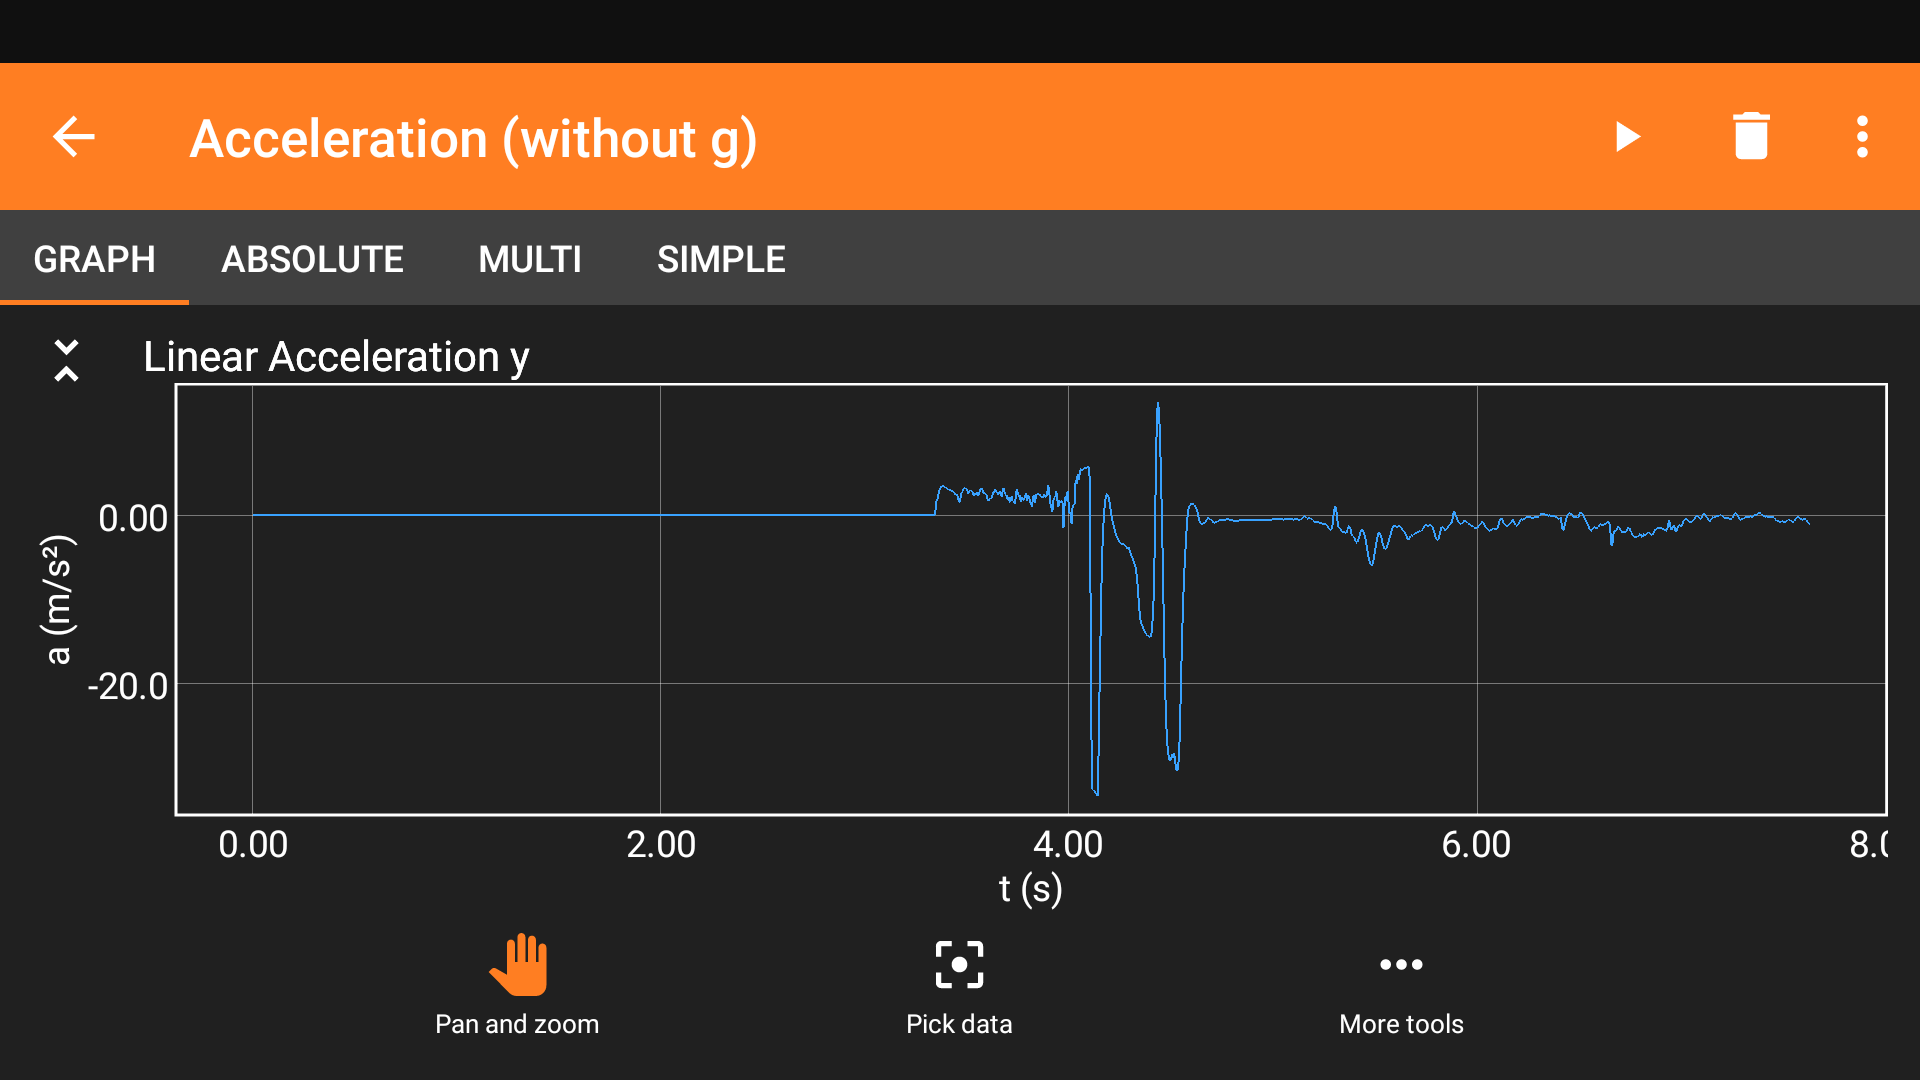
\includegraphics[width=\textwidth]{phyphox}
  \caption{Uno \emph{screenshot} della schermata dello strumento
           \emph{Acceleration (Whitout g)}
           nell'applicazione Phyphox.}
  \label{fig:phyphox}
\end{figure}

In seguito il professore assegna agli studenti un compito da eseguire
a casa: indica agli studenti di scegliere una superfice inclinata
e priva di attrito
\footnote{
          Si ricorda che gli studenti di una classe prima liceo
          non hanno familiarità con il concetto di attrito,
          dunque il professore dovrebbe utilizzare termini differenti
          come ``Superficie inclinata e liscia''.
         },
e di far scivolare il telefono lungo la superficie, attivando
la registrazione dati dello strumento appena mostrato.
Il compito di scegliere l'inclinazione del piano, il modo in cui
collocare il telefono sopra di esso, e altre osservazioni pratiche
sono lasciate allo studente.

Durante la lezione successiva l'insegnate chiede agli studenti
di condividere la propria esperienza e di spiegare l'interpretazione
che questi danno ai grafici prodotti dall'applicazione.
Il docente dovrebbe aver riprodotto l'esperienza, in modo
da poter presentare agli studenti i propri risultati in una
forma più adatta alla comprensione degli stessi.
Si ritiene che grafici prodotti da Phyphox siano utili,
in quanto immediati, ma di difficile interpretazione
per uno studente. Il docente potrà esportare i propri
dati nel formato preferito grazie alla funzione
\emph{Export Data}, e in seguito analizzarli con uno
strumento di propria scelta.
Una possibile analisi è mostrata nella Figura \ref{fig:a_phyphox}.


\begin{figure}[H]
\centering
  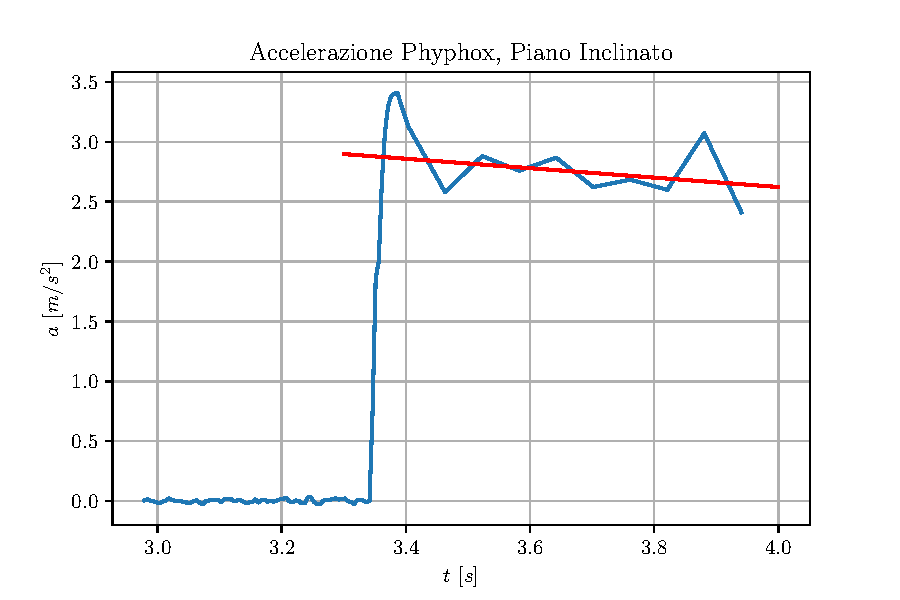
\includegraphics[width=\textwidth]{a_phyphox}
  \caption{Il plot, realizzato con il modulo \emph{Matplotlib}
           del linguaggio di programmazione \emph{Python},
           mostra l'accelerazione lungo il piano misurata da
           Phyphox. I dati sono stati mediati nel tempo
           per rimuovere il rumore e un fit lineare è stato
           eseguito sulla coda.
          }
  \label{fig:a_phyphox}
\end{figure}

Il professore aiuta gli studenti ad analizzare il grafico ponendo
alcune domande: ``Riuscite ad individuare nel grafico l'istante
in cui il telefono è stato lasciato libero di scivolare?'',
``Quando vale l'accelerazione prima che il telefono inizi a
scivolare?'', ``Quanto vale l'accelerazione nell'istante
in cui il telefono viene lasciato scivolare, ma è ancora fermo,
ovvero la sua velocità vale zero?'', ``E mentre il telefono sta
scivolando?''. In questo modo egli guida gli studenti verso
la realizzazione che un corpo avente velocità nulla ad un certo
istante, non necessariamente deve avere anche un'accelerazione nulla.

\appendix
\chapter{Analisi Dati}
\section{Moto Rettilineo Uniforme}

\begin{figure}[H]
\centering
  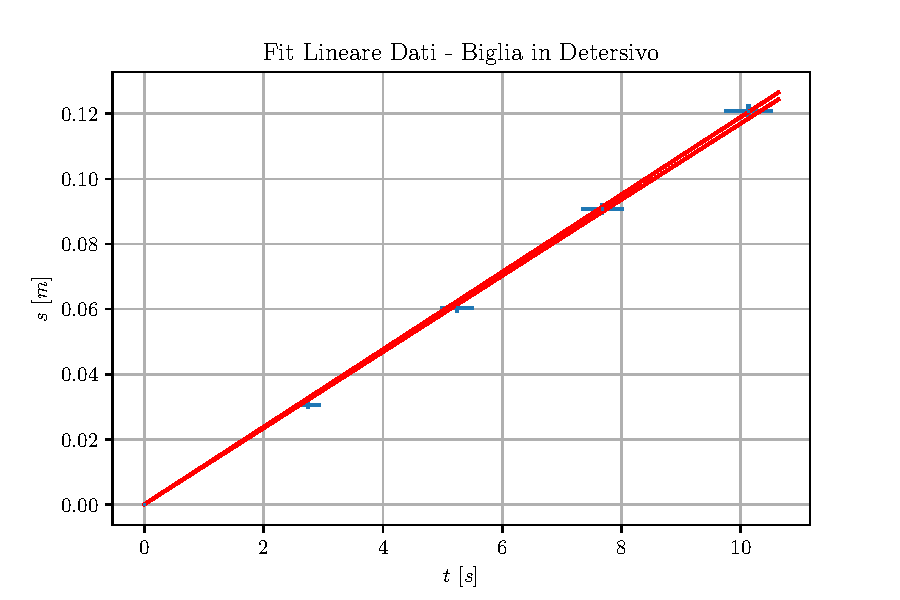
\includegraphics[width=\textwidth]{fit_marble}
  \caption{Fit lineare dei dati per l'esperimento della biglia che cade nel detersivo,
           un esempio di moto rettilineo uniforme.}
  \label{fig:fit_marble}
\end{figure}

\begin{table}[H]
  \renewcommand{\arraystretch}{1.5}
  \centering
  \begin{tabular}{ | c | }
    \hline
    $v$ [$m/s$] \\
    \hline
    $0.01180\pm0.00010$ \\
    \hline
  \end{tabular}
  \caption{Valore atteso ed errore della velocità da fit con il metodo dei minimi
           quadrati.}
  \label{tab:fit_marble}
\end{table}

\section{Moto Rettilineo Uniformemente Accelerato}

\begin{figure}[H]
  \centering
  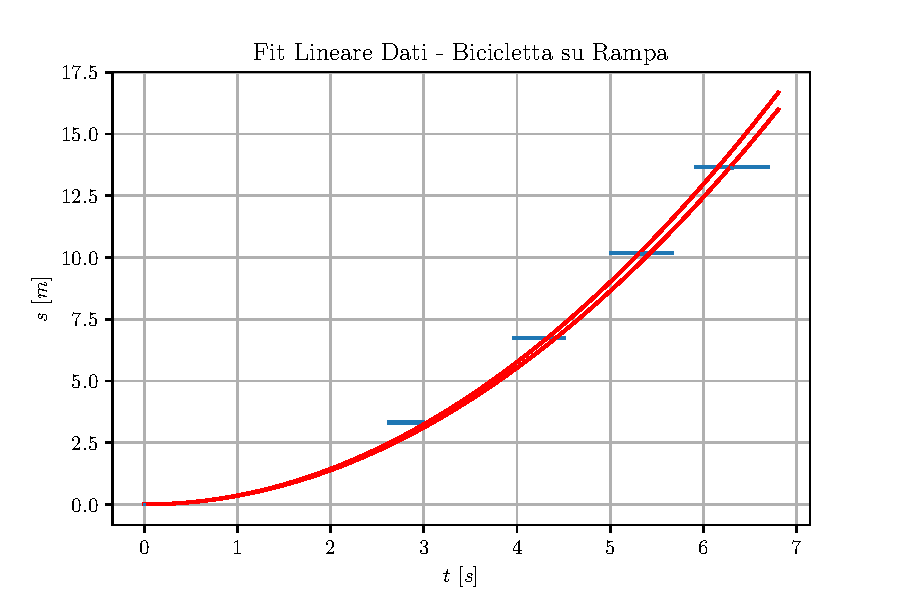
\includegraphics[width=\textwidth]{fit_bike}
  \caption{Fit lineare dei dati per l'esperimento della bicicletta che scende da una rampa,
           un esempio di moto rettilineo uniformemente accelerato.}
  \label{fig:fit_bike}
\end{figure}

\begin{table}[H]
  \renewcommand{\arraystretch}{1.5}
  \centering
  \begin{tabular}{ | c | c | c | }
    \hline
    $a$ [$m/s^2$] &  $\theta$ [deg] & pendendenza [\%] \\
    \hline
    $0.706\pm0.015$ & $4.13\pm0.09$ & $7.21\pm0.15$ \\
    \hline
  \end{tabular}
  \caption{Valore atteso ed errore dell'accelerazione, dell'angolo di inclinazione della rampa
           e della pendenza percentuale da fit con il metodo dei minimi quadrati.}
  \label{tab:fit_bike}
\end{table}

\bibliography{bibliografia}{}
\bibliographystyle{plain}
\addcontentsline{toc}{chapter}{Riferimenti}

\end{document}
